
%
\documentclass[%
 reprint,
 amsmath,amssymb,
 aps,
]{revtex4-1}

\usepackage{graphicx}% Include figure files
\usepackage{dcolumn}% Align table columns on decimal point
\usepackage{bm}% bold math


\begin{document}



\title{Sistema de Gestion para el concurso de Proyectos de la EPIS}
\author{Jose Pastor Mendoza}
\author{Arlyn Cotrado Coaquira}
\author{Andrés De La Barra Vasquez}
\affiliation{%
 Universidad Privada de Tacna \textbackslash Facultad de Ingenieria \textbackslash Escuela Profesional de Ingenieria de Sistemas
}%

\begin{abstract}
\begin{center}
\textbf{Resumen}
\end{center}
Balanced Scorecard y Business model canvas son técnicas de análisis empresarial . Ambas técnicas son útiles para mejorar el desempeño organizacional. Pero sus aplicaciones difieren. Ambos se pueden usar junto con los indicadores clave de rendimiento para monitorear y mejorar el rendimiento de la organización. Vamos a entender tanto la técnica en detalle.


\begin{center}
\textbf{Abstract}
\end{center}
Balanced Scorecard and Business model canvas are business analysis techniques. Both techniques are useful to improve organizational performance. But their applications differ. Both can be used together with the key performance indicators to monitor and improve the performance of the organization. We will understand both the technique and the detail.

\end{abstract}



\maketitle

%\tableofcontents

\section {Introducción}

El BSC retiene las medidas financieras tradicionales que se combinan con la metodología del EVA y se complementan con indicadores de desempeño futuro.\\
Ésta es una metodología útil para la implementación estratégica que “traduce” la misión, la visión y la estrategia de las diferentes unidades de negocio de la\\
empresa en objetivos e indicadores tangibles, los cuales son agrupados en forma de causa y efecto, en cuatro perspectivas que permiten visualizar el desempeño\\
organizacional: perspectiva financiera, clientes, procesos internos y crecimiento y aprendizaje.\\

El BSC sugiere que las medidas financieras y no financieras deben ser parte del sistema de información para los empleados de todos los\\
niveles de la organización. Aquellos de niveles inferiores podrán entender el efecto financiero de sus decisiones, mientras que los de niveles superiores podrán\\
entender los impulsores del efecto financiero a largo plazo.\\


%-----------------------------------------------------------------
\section {Objetivos}
\begin{itemize}
\item Integrar todas las actividades involucradas en el proceso del concurso de proyectos de la EPIS. \\
\item Facilitar a todos los usuarios el proceso que les corresponda realizar segun su rol. \\
\item Investigar el uso de tecnologias web para la realizacion del proyecto.  \\
\item Crear un producto completo para mejorar tiempos y organizar procesos .\\
\end{itemize}

\section {Problematica}
No tener un estructura definida en los concursos liberados en la universidad privada de tacna, la necesidad de poder gestionarlo con más herramientas y más procesos se ve necesaria para poder establecer informes y un control avanzado de ello. 
Se converso con la ingeniería Liliana respecto a la problemática respecto a la gestión del concurso de proyectos de la EPIS y nos indico que actualmente no se cuenta con un sistema especifico para esta actividad, por lo que deben recurrir al uso de Excel, Gmail, un software online solo para realizar sorteos, asi como también implementar algunas funciones extras para realizar la calificación de proyectos por parte de los jurados y sobretodo, unificar estos procesos.

\section {Desarrollo de la solucion}

La presente propuesta plantea:
\begin{itemize}
    \item Realizar una aplicación web que contenga 3 vistas: 1 para los estudiantes, otra para el administrador del concurso de proyectos (Ingeniera Liliana) y otra para los jurados.
     \item Para la vista del estudiante, tendrá que crearse una cuenta , luego tendrá una vista sobre información respecto al concurso de proyectos(documentos que necesite) y también, un modulo para subir toda la documentación y registrar su proyecto que será enviado a evaluar por el administrador.
     \item Para la vista del administrador, tendrá un modulo para ver las solicitudes de los proyectos que desean registrarse para participar. Tendra otro modulo para organizar que categorías y que cursos van a participar. Otro modulo será para agregar a los jurados para cada categoría. Otro modulo para hacer un seguimiento de votos. 
    \item Para la vista del jurado, solo tendrán el modulo para votar según la categoría a la que esten asignados.
    \item Tambien se plantea agregar un chatbot al Facebook de Tutoria Epis, la cual se encargara de dar información histórica sobre el concurso de proyectos (referido a información del pasado sobre los ganadores de anteriores ediciones, nombres de proyectos que hayan participado).
\end{itemize}
	
\begin{center}
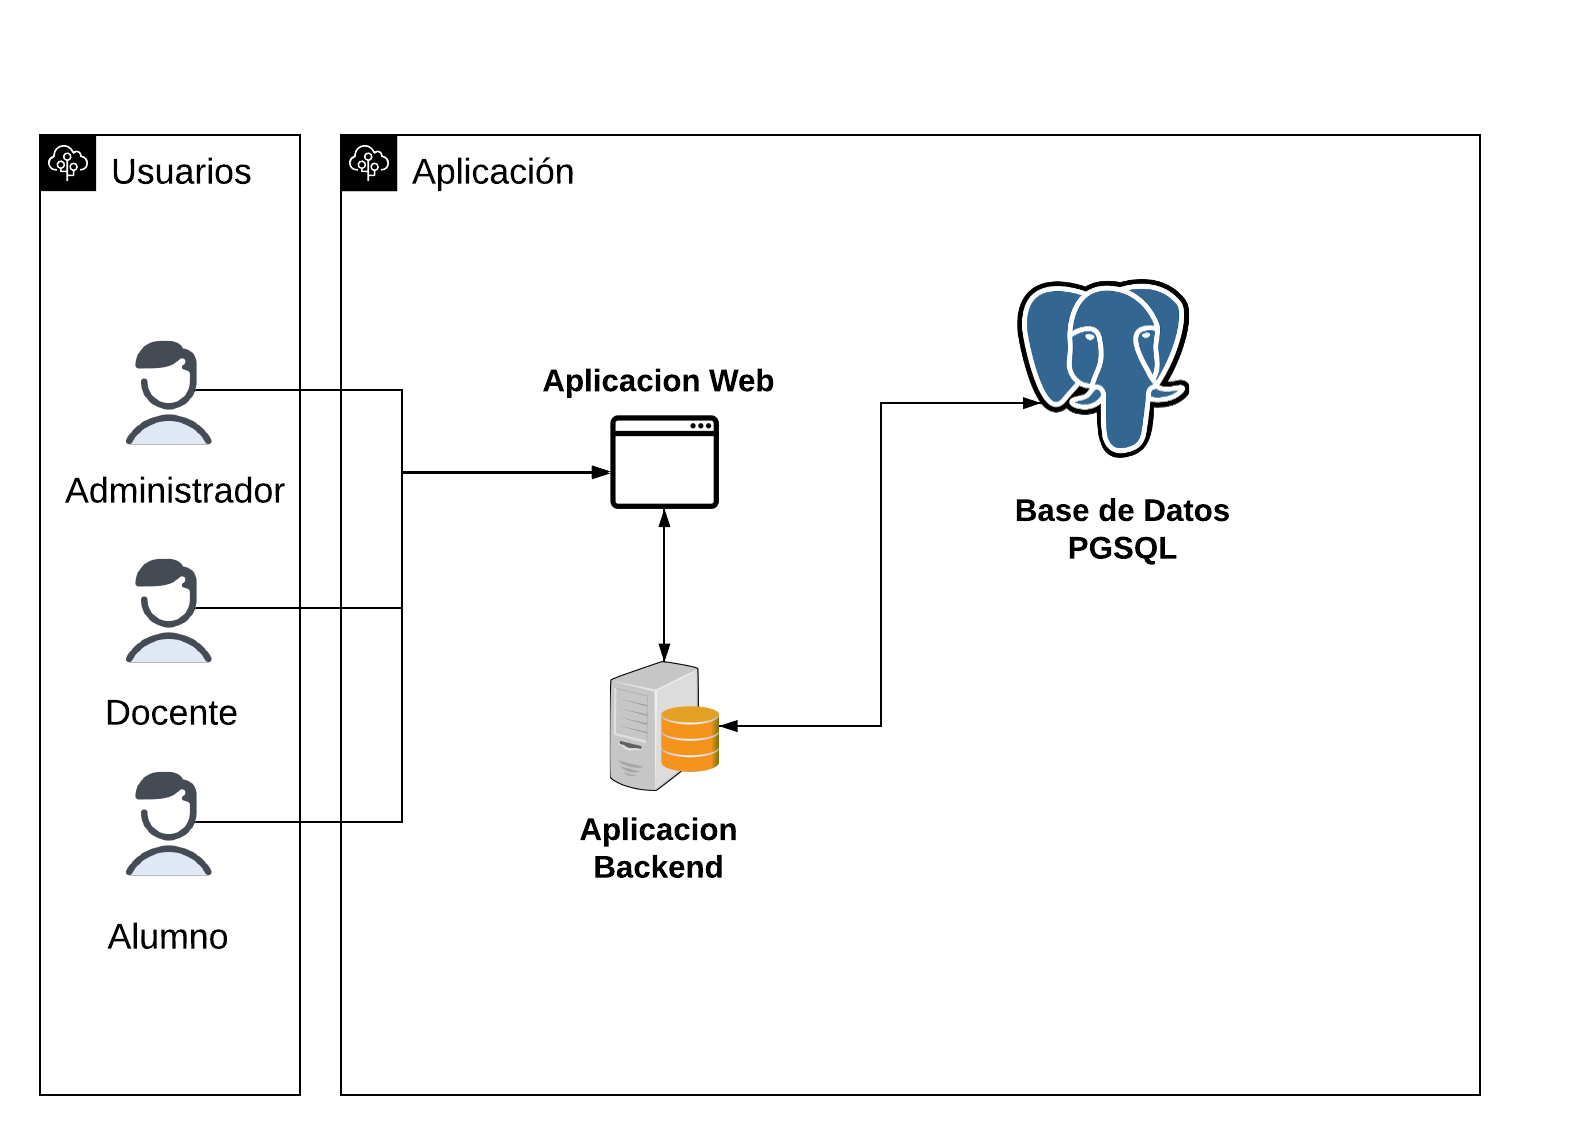
\includegraphics[width=10cm]{./Imagenes/aq}
\end{center}

%-----------------------------------------------------------------
\section{Conclusiones}

\begin{itemize}
\item El Balanced Scorecard nos ayuda a establecer y enfocar las estratégias de la empresa hacia el futuro, todo con el fin de poder convertir en realidad la visión empresarial, esto se logra a través de la suma de los objetivos de cada una de las cuatro perspectivas que nos propone mejorar el BSC.

\item Balanced Scorecard y Business model canvas son técnicas de análisis empresarial. Ambas técnicas son útiles para mejorar el desempeño organizacional. . Ambos se pueden usar junto con los indicadores clave de rendimiento para monitorear y mejorar el rendimiento de la organización. 

\end{itemize}

% Bibliografia.
%-----------------------------------------------------------------

%\bibliographystyle{plain}
%\bibliography{Bibliografia}

\end{document}

